%-------------------------------------------------------------------------
% Design Project Input/Output Module Description
%-------------------------------------------------------------------------

\clearpage
\section{Water Input Module}
\label{sec-input-water}

This input module enables your IoT device to sense the level of water in
the environment using a water sensor called eTape. Water level sensing
can play an important role in environmental monitoring systems, disaster
warning, cooling systems, water purification, medical equipment care,
etc. This tape can easily be secured to a street pole, hung on the wall
of a room, or attached to the side of a water container or other similar
environments. The tape is a variable resistor. When immersed in water,
the sensor tape is compressed from both sides by hydrostatic pressure,
and the tape's resistance varies as the water level rises and falls. The
resistance and water level are inversely proportional: the lower the
water level, the higher the output resistance; the higher the water
level, the lower the output resistance.  The Arduino cannot directly
sense resistance, but it can sense an analog input voltage. We will use
a simple circuit called a voltage divider so that the voltage across the
water sensor is proportional to the resistance.

A sample circuit and Arduino code is shown below to get you started.
The circuit places a \wu{560}{$\Omega$} resistor in series with the
water sensor so that voltage is divided between the two components. A
\wu{560}{$\Omega$} resistor has green-blue-purple bands. We use a wire
to connect the node in between the resistor and the water sensor to an
analog input of the Arduino so that the Arduino can read the voltage
from one end of the \wu{560}{$\Omega$} resistor to ground. Use long
wires to connect the water sensor to the breadboard so that you can
freely move the sensor away from the Arduino and breadboard (which
should not get wet!). The example code will print the analog reading
from the water level sensor on the serial monitor, similar to how we
printed the analog reading from the grayscale sensor in Lab~2. After
setting up the circuit and programming the Arduino, open the serial
monitor and check the value of the water level sensor when dipped in a
container of water. Be careful not to get the top electrical leads of
the sensor wet. Try dipping the water level sensor further into the
water. What happens to the reading and why do you think this happens?

\vspace{0.1in}
\begin{minipage}[t]{0.49\tw}
  \vspace{0pt}

  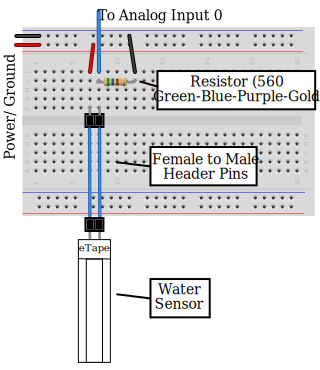
\includegraphics[width=\tw]{input-water-annotated.svg.pdf}
\end{minipage}
\hfill
\begin{minipage}[t]{0.49\tw}
  \vspace{0.1in}
  \begin{Verbatim}[gobble=3,fontsize=\small]
    int pin_water = A0;

    void setup() {
      Serial.begin(9600);
      pinMode( pin_water, INPUT );
    }

    void loop() {
      int water_level = analogRead( pin_water )

      Serial.println( water_level );
      delay(1000);
    }
  \end{Verbatim}
\end{minipage}
\vspace{0.1in}

%Questions:
